\chapter{Energy-based Multi-Modal Attention} 
\label{chapter-emma} 

The literature review (Chapter \ref{chapter-literature-review}) showed that previous research in MMDL has been mostly focused on leveraging multi-modality to improve the accuracy of the predictions. In this chapter, a new attention module is presented to increase the robustness against failing modes: as long as at least one modality provides sufficient information for the task at hand, the prediction network will be able to perform well. First, we start by providing a conceptual general framework. Then, the design of each step of the framework is described. Finally, the training of EMMA is discussed, along with two novel regularizers. 

%----------------------------------------------------------------------------------------
%	SECTION 
%----------------------------------------------------------------------------------------

\section{General Framework}\label{sec:general-framework}

A typical multi-modal network (MMN) receives samples at its input, where each sample is composed of multiple modes such as images and sounds. In real-world applications, the relative informativeness of different modes may evolve over time, on a per sample basis, e.g. as a result of perturbations or sensor malfunctions. 

In order to address this problem, an attention module is proposed that pre-processes each input sample and evaluates the relative informativeness, also referred to as importance, of each mode. More precisely, those modes deemed informative are assigned a high weight, typically close to 1, whereas the modes considered too uninformative are assigned a weight close to 0. The weighted modes are then fed to the MMN.

The interpretation of the role of EMMA is twofold. First, EMMA can be seen as a sort of gate filtering out perturbations. Indeed, failing modes can provoke high activations in the MMN, thus affecting its predictive performance negatively. Masking the failing modes allows to diminish these activations, thereby improving predictions quality. Another way to view it is to understand that the MMN model is able to extract the multiplied weight from the original input. The model can then learn to make more robust predictions based on the extra information provided by that weight. Notice that even tough the internal architecture of the MMN is often structured as a many-to-one encoder-decoder as discussed in Section \ref{sec:mmdl}, the EMMA module can be fitted to any MMN architecture.

The key concept on which EMMA relies to produce scores for different modes is that of modal importance\footnote{Introduced in Section \ref{sec:proposed-solution}}. As a reminder, the modal importance is defined in terms of three intrinsic and related properties of each mode, namely
\begin{itemize}
\item \textit{relevance}: the intrinsic informativeness of the mode for the predictive task at hand.
\item \textit{failure intensity}: the propensity of a mode to trigger undesirable activations in the neural network.
\item \textit{coupling}: the interdependencies between the modes, which describe the extent to which the mode provide independent, complementary, redundant or conflicting information.
\end{itemize}
The EMMA module will essentially try to learn the relationships between these properties for a specific dataset. 

\begin{figure}[!ht]
\vspace*{5mm}
\centering
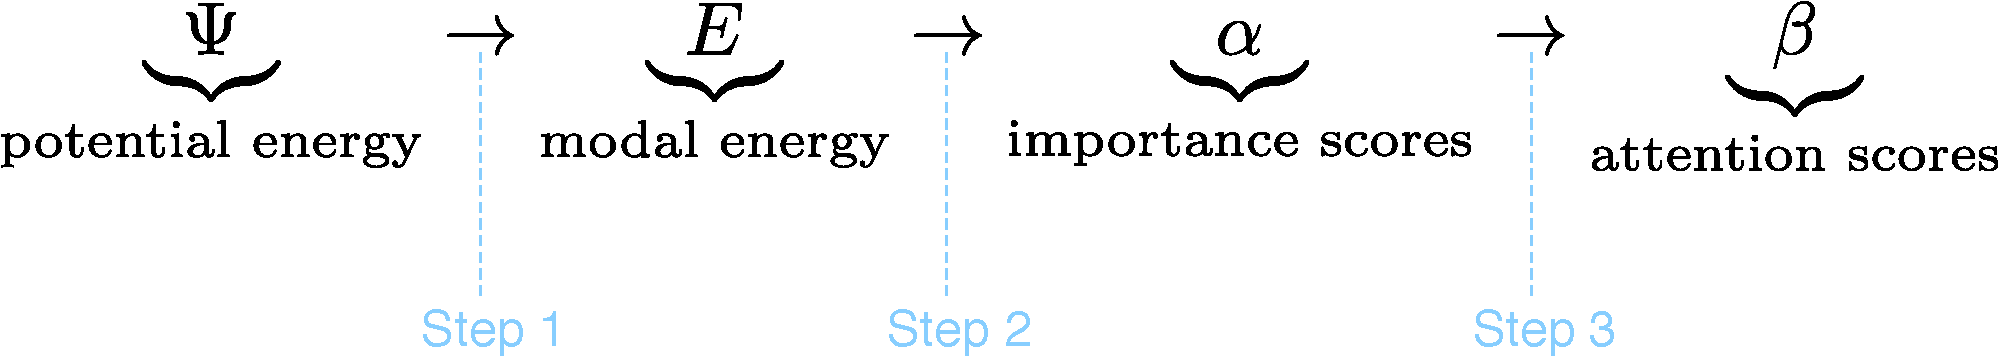
\includegraphics[scale=0.4]{figures/framework}
\caption[Summary of main steps in EMMA]{Summary of main steps in EMMA (step 2, 3 and 4 are detailed in the following sections, step 1 was explained in Chapter \ref{chapter-energy-estimation})}
\label{fig:framework}
\end{figure}\vspace*{5mm}

For the sake of clarity, making the exposition more formal is now in order. Let $\mathcal{D}^{N} = \{(\mathbf{X}_1,  y_1), \ldots, (\mathbf{X}_N, y_N)\}$ be a dataset of i.i.d. samples, where the input $\textbf{X}_k$ is composed of $M$ modes $\{\mathbf{x}_1, \ldots, \mathbf{x}_M\}$. The MMN tries to make predictions $\hat{y}_k$ as close as possible to the groundtruth $y_k$. The EMMA module computes the importance of mode $i$ starting with the failure intensity, which is measured by the potential energy $\Psi_i = \Psi(\mathbf{x}_i)$ (step 1 in Figure \ref{fig:framework}, previously motivated in the introduction of Chapter \ref{chapter-energy-estimation}). To capture the two other modal properties, namely the modal relevance and coupling, two additional functions are introduced. On the one hand, the \textit{self-energy} $e_i$ is designed to spontaneously learn the relationship between the relevance and the failure intensity. This comes as a result of the fact that it is a function of $\Psi_i$ and its parameters are optimised with respect to the loss on the predictions. On the other hand, shared energies $e_{ij}$ are designed to capture the optimal coupling between modes. Using these functions, the \textit{modal energy} $E_i$ can be constructed such that it takes a low value if mode $i$ is important and a high value otherwise (step 2 in Figure \ref{fig:framework}, further discussed in Section \ref{sec:step2}). Next, the modal energies are normalized via the Boltzmann distribution\footnote{See Section \ref{sec:ebm}} to form \textit{importance scores} $\alpha_i$, which are scalar values between zero and one, with more important modes corresponding to higher values (step 3 in Figure \ref{fig:framework}, further discussed in Section \ref{sec:step3}). From each importance score, the model then determines an \textit{attention score} $\beta_i$, which is representative of the amount of attention that should be paid to each mode by the MMN (step 4 in Figure \ref{fig:framework}, further discussed in Section \ref{sec:capacity}). Finally, each mode is multiplied by its respective attention score (step 5 in Figure \ref{fig:framework}). Section \ref{sec:capacity} will clarify why the modes are not directly multiplied by the importance scores instead.  A high-level view of the attention module EMMA is illustrated in Figure \ref{fig:mnn-with-emma}. The next sections detail the form and specificities of each function introduced previously.

\begin{figure}[!h]
\centering
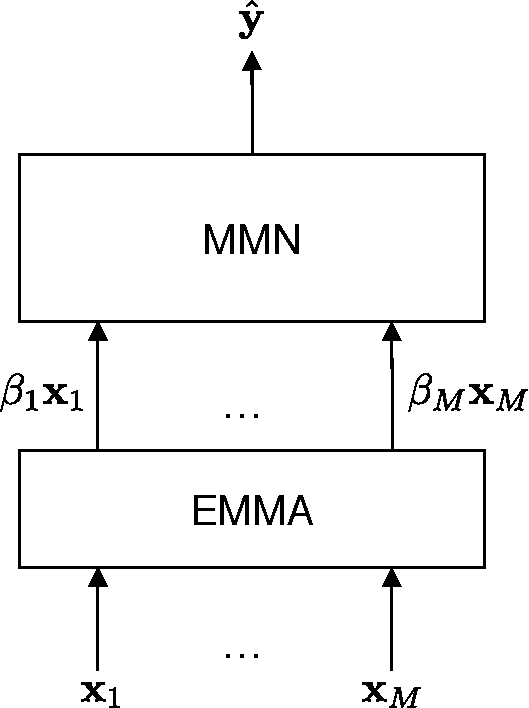
\includegraphics[scale=0.5]{figures/mlp-with-emma}
\caption[High-level view of a Multi-Modal Network with EMMA]{High-level view of a Multi-Modal Network with the EMMA module.}	
\label{fig:mnn-with-emma}
\end{figure}

%----------------------------------------------------------------------------------------
%	SECTION 
%----------------------------------------------------------------------------------------

\section{From Potential to Modal energies (step 2)}\label{sec:step2}
The self-energy is defined as an affine function of the potential energy,
\begin{equation}
e_i = w_i\Psi_i + b_i \qquad \text{with} \qquad w_i \in [1, +\infty],\, b_i \in \mathbb{R}^+,
\label{eq:self-energy}
\end{equation}
where the parameters $w_i$ and $b_i$ are trained via a loss function on the predictions. Therefore, the model is able to capture both the relevance and failure via the self-energy. The second advantage of this transformation is that it helps the module to handle potentials on different numerical scales. Indeed, Equation (\ref{eq:potential-prop}) only guarantees being proportional to the NLL, thus potentials of different modes may not be on comparable scales. The reason the parameters are constrained to be positive will be justified below. Additionally, it will be shown below that self-energies are guaranteed to be positive at the end of this section.

After computing the self-energies, the shared energies can be determined. The expression $e_{ij}$ denotes the shared energy of mode $j$ on $i$ and is constructed from the self-energies as follows
\begin{equation}
e_{ij} = w_{ij}e_i^{\gamma_{ij}}e_j^{1-\gamma_{ij}} \qquad \text{with} \qquad w_{ij} \in [-1,+1],\,\, \gamma_{ij} \in [0,1]
\label{eq:shared-energy}
\end{equation}
where the parameter $\gamma_{ij}$ learns the degree of coupling in the spectrum from strongly coupled ($\gamma_{ij}=0$) to independent ($\gamma_{ij} = 1$). Indeed, if the model learns a value of $\gamma_{ij}$ close to zero, mode $j$ will influence mode $i$ much more than for a $\gamma_{ij}$ close to unity. Equally important is the direction of coupling between mode $i$ and $j$, determined by the weights $w_{ij}$ and $w_{ji}$. We verify that an increase/decrease of the self-energy $e_j$ leads to an increase/decrease of the modal energy $E_i$ for a positive weight $w_{ij}$, and a decrease/increase of $E_i$ for a negative weight $w_{ij}$. This is valid since self-energies are guaranteed to be positive (see next paragraph). The direction of coupling is useful to distinguish modes with redundant or conflicting information from those with complementary information. Notice that the degree and direction of coupling are asymmetric ($\gamma_{ij} \neq \gamma_{ji},\, w_{ij} \neq w_{ji}$). This asymmetry is justified by the following example: take a multi-modal problem with three modes A, B and C. We want the model to learn that if mode A is failing, it is optimal that mode B "takes over". And if mode B is failing, it is optimal for C to "take over". This example can only be modelled with asymmetry. In conclusion, the model has the ability, through the use of shared energies, to discover the different interdependencies between the modes.

A consequence of the design of Equation (\ref{eq:shared-energy}) is that the evaluation of the gradient during the backpropagation step now involves taking the logarithm of $e_i$\footnote{See Appendix \ref{sec:log-gradient}}, which is undefined for negative values. As the weights in Equation (\ref{eq:self-energy}) are positive, we only have to make sure the values of the potential energy are positive. The latter is done by lowering the potential $\Psi_i$ to Euler's number $\mathrm{e}$ as
\begin{equation}
\Psi_i \leftarrow \max(\mathrm{e}, \Psi_i - \Psi_i^{(\text{min})} + \mathrm{e})
\label{eq:correction}
\end{equation}
where $\Psi_i^{(\text{min})}$ denotes the lowest value of $\Psi_i$ in the training set. This correction avoids undefined values ($\Psi_i \geq 0$), exploding gradient\footnote{Exploding gradients are very large gradients, which in turn results in large updates of the network weights, resulting in an unstable network. A good overview on this subject can be found in \citep{exploding}} ($\Psi_i \geq \mathrm{e}$) and guarantees self-energies to be positive. The reason a max-operator is used is because lower energy values than $\Psi_i^{(\text{min})}$  can occur during inference. Clearly, this correction step (\ref{eq:correction}) must be performed prior to the computation of self-energies (\ref{eq:self-energy}).

%----------------------------------------------------------------------------------------
%	SECTION 
%----------------------------------------------------------------------------------------

\section{From Modal energies to Importance scores (step 3)}\label{sec:step3}
The importance scores are computed from the modal energies via the Boltzmann distribution:
\begin{equation}
\alpha_i = \frac{1}{Z}e^{-\rho E_i} \quad \text{with the partition function} \quad Z = \sum_{j=1}^M e^{-\rho E_j} 
\label{eq:gibbs-distrib}
\end{equation}
This guarantees the scores are normalized and sum up to one. A mode $i$ will be said to be important if its score is close to one (low modal energy $E_i$). The hyperparameter $\rho$ represents the coldness, the inverse of the temperature. It controls the entropy of the importance scores distribution. At high temperature ($\rho \rightarrow 0$) the distribution becomes more uniform, and at low temperature ($\rho \rightarrow +\infty$) the importance scores corresponding to the lowest energy tends to 1, while the others approach 0. As can be observed in Figure \,\ref{fig:gibbs}, the coldness has a significant influence on the overall behaviour of the attention module. Hence, careful tuning of $\rho$ is required.

\begin{figure}[!h]
\centering
\begin{subfigure}{.5\textwidth}
  \centering
  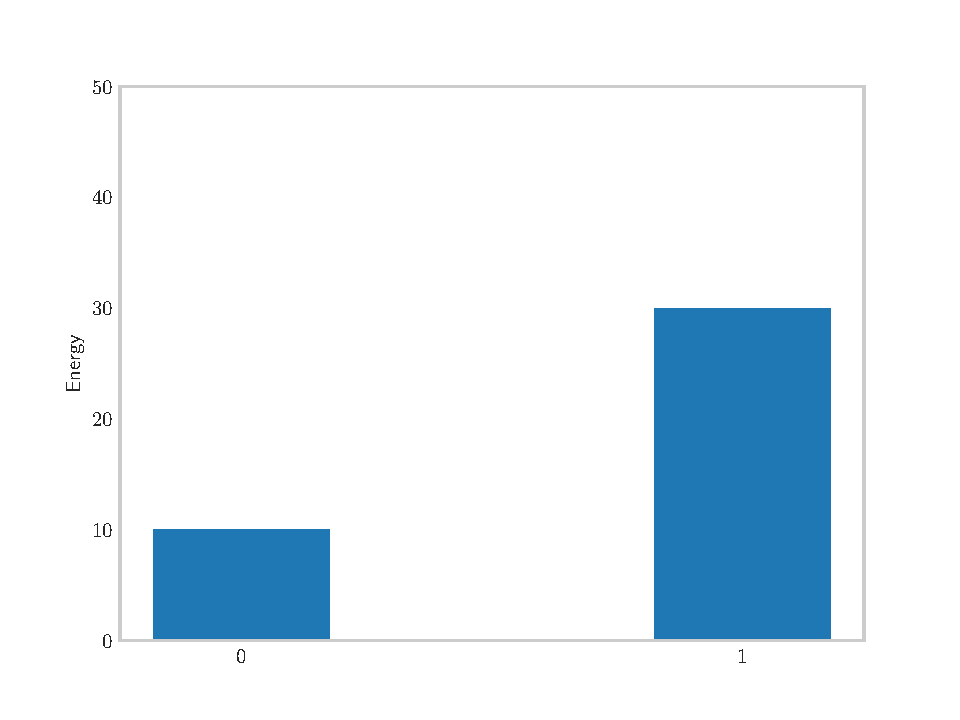
\includegraphics[width=.95\linewidth]{figures/input-gibbs}
  \caption{Energies}
\end{subfigure}%
\begin{subfigure}{.5\textwidth}
  \centering
  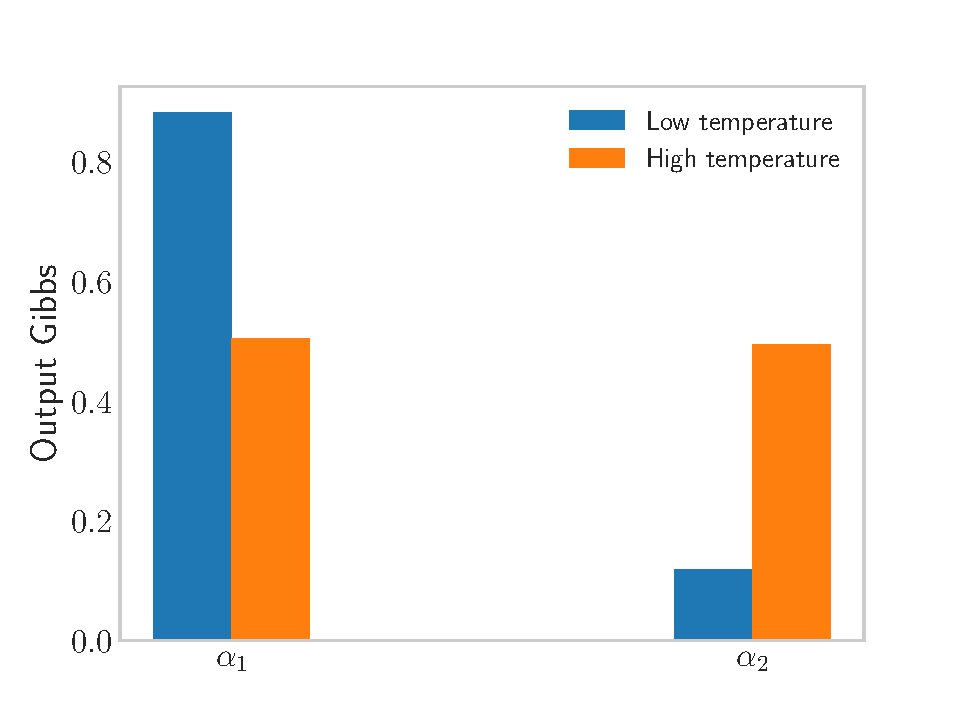
\includegraphics[width=.95\linewidth]{figures/result-gibbs}
  \caption{Importance scores}
\end{subfigure}
\caption[Input-output of Boltzmann distribution for two different temperatures]{Input-output of Boltzmann distribution for two different temperatures, low temperature ($\rho = 0.1$) and high temperature ($\rho = 0.001$)}
\label{fig:gibbs}
\end{figure}


%----------------------------------------------------------------------------------------
%	SECTION 
%----------------------------------------------------------------------------------------

\section{From Importance to Attention scores (step 4)}\label{sec:capacity}
The attention scores are given by
\begin{equation}
\beta_i = \max[0, \tanh(g_a\alpha_i - b_a)] \quad \text{with} \quad g_a > 0,\,\,b_a\in [0,1]
\end{equation}
The hyperbolic tangent adds non-linearity while the gain $g_a$ and bias $b_a$ enable the model to control the threshold and capacity (see Figure \ref{fig:attention-function}). Those two concepts are detailed below.
\begin{figure}[!h]
\centering
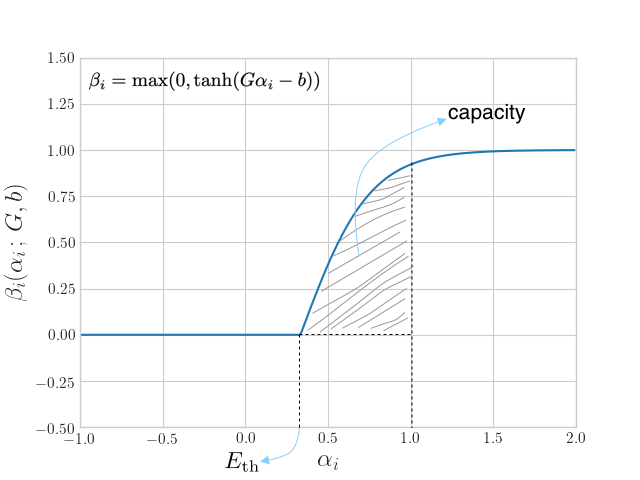
\includegraphics[scale=0.5]{figures/tanh-annotated}
\caption[Attention function]{Attention function (the max-operator generalizes the attention function to cases where $\alpha \in \mathbb{R}$)}
\label{fig:attention-function}
\end{figure}

\subsection*{Energy threshold}
The module will let the information of mode $i$ pass by, only if $g_a\alpha_i - b_a > 0$
\begin{equation}
\begin{split}
&\Leftrightarrow\log(\alpha_i) > \log(b_a/g_a)\\
&\Leftrightarrow E_i \leq \frac{\log(g_a/b_a) - \log(Z)}{\rho} = E_{\text{threshold}}
\end{split}
\end{equation}
where $E_{\text{threshold}}$ represents the maximum energy level for mode $i$ to be taken into account (see Figure \ref{fig:attention-function}). We deduce that the learned gain and bias control this threshold. Notably, the threshold is varying on a per-sample basis due to the partition function $Z$. For example, an increase of the overall perturbation level on the entire input results in a reduction of the partition function, leading to a higher threshold $E_{\text{threshold}}$. It can thus be deduced that EMMA becomes less selective if the overall quality of the sample decreases. 

\subsection*{Capacity}
A more common way to write the attention function would be $\tanh(\mathbf{W}\bm{\alpha}+\mathbf{b})$, whereas we have $\tanh(g_a I\bm{\alpha}-b_a\mathbf{1})$, where $I$ is the identity matrix. We argue the latter better mimics human's attention, permitting us to introduce the concept of capacity, which in psychology is viewed as the amount of resource that can be allocated \citep{attention-is-effort}. If we look at Figure \ref{fig:attention-function}, this can be translated as,
\begin{equation}
\text{capacity} \triangleq \int_0^1 \tanh(g_a\alpha - b_a)d\alpha 
\end{equation}
Define the auxiliary variable $u = g_a\alpha - b_a$. Now using
\begin{equation}
\frac{du}{d\alpha} = g_a \Leftrightarrow d\alpha = \frac{1}{g_a}du
\end{equation}
we can write 
\begin{equation}
\begin{split}
\text{capacity} &= \frac{1}{g_a} \int_{-b_a}^{g_a-b_a} \tanh(u)du  \\
&= \frac{1}{g_a}\log[\cosh(u)]\bigg\rvert_{-b_a}^{g_a-b_a} + \cancel{\text{constant}} \\
&= \frac{1}{g_a}\log\bigg[\frac{\cosh(g_a - b_a)}{\cosh(-b_a)}\bigg]
\end{split}
\label{eq:capacity}
\end{equation}
When the capacity is too low, no sufficient amount of information is passed to the MMN, leading to wrong predictions. Similarly, if the capacity is too high, the perturbations of the failing modes will pass and cause a decrease in performances. It is expected that the model learns the optimal trade-off. However, if we want the attention module to be robust against failing situations it was not trained on, we suggest minimizing capacity would result in appealing properties for the system as a whole. The reasons for minimizing the capacity are two-fold: it forces the module to mask out more information, which may be sub-optimal on the training set but useful to generalize against more intensive failing modes. The second reason is to avoid the extreme case where the module leaves all the inputs unchanged (maximal capacity) and instead it is the MMN who learns to suppress perturbations. The ideal method for controlling the capacity, would be to add the derived expression (\ref{eq:capacity}) as a regularizer to the loss function, but this could potentially lead to instabilities\footnote{The gradient of Equation (\ref{eq:capacity}) can become very large for certain values of its weights $g_a$ and $b_a$.} during training. A less precise but more stable way is to introduce the expression $g_a-b_a$ instead in the loss function. We verify that minimizing this expression will minimize the gain while maximizing the bias, i.e. lead to a decrease of the capacity. Nevertheless, Equation (\ref{eq:capacity}) can still be used to compute the learned capacity of the module. Notice that the concept of capacity can also be applied to $\tanh(W\bm{\alpha}+\mathbf{b})$, but in this case each mode would have his own capacity, making the importance scores less meaningful.


%----------------------------------------------------------------------------------------
%	SECTION 
%----------------------------------------------------------------------------------------

\section{Training \& Regularization}\label{sec:regul}
The training of the attention module and the prediction model is performed in two stages (see Figure \ref{fig:training}). First, each mode is assigned a separate autoencoder, which is trained on the mode to learn the potential energy function. Once trained, the weights of the autoencoders are frozen. In the second phase, EMMA is inserted in front of the MMN and is trained end-to-end on both normal and corrupted data. By corrupted data, we mean samples on which a corruption process is applied in order to simulate one or more failing modes. Notably, the computational overload induced by the training of EMMA in the second stage is often negligible with respect to the MMN, provided that the number of parameters of EMMA\footnote{The number of parameters of EMMA scales up quadratically with the number of modes.} is in most cases far less than the number of parameters of the MMN. 

Additionally, two regularizers are introduced in the loss function, written as
\begin{equation}
\tilde{\mathcal{L}} = \mathcal{L}(y,\hat{y}) + \lambda_c(g_a-b_a) - \lambda_e \Omega \quad \text{with} \quad \Omega = \sum_{k=1}^M \xi_k \log(\alpha_k) \quad \text{and} \quad \xi_k = \begin{cases}
      \xi_- = -1 & \text{if}\ \mathbf{x}_k\, \text{is corrupted} \\
      \xi_+ = +1 & \text{otherwise}
    \end{cases}
\label{eq:regularization}
\end{equation}
with $\lambda_c$ and $\lambda_e$ being positive real numbers used to set the relative importance of each regularizer, and the $\xi_k$ vector being manually encoded. The first regularizer minimizes the capacity, where a higher $\lambda_c$ pushes the module to let less information pass through in general (i.e., to be more "cautious"). The second regularizer ($\lambda_e \Omega$), which we call the energy regularizer, controls the trade-off between on the one hand the coupling and on the other hand the failure intensity. In use-cases with complex asymmetric interactions between the modes, the shared energies could potentially cause large discrepancies between modal energies $E_i$ and their original potential energies $\Psi_i$. A major drawback of having such discrepancies is that this leads to a reduction of the influence of the failure intensity in the computation of the attention scores. This may result in poor generalization to samples with more intensive failing modes. We show that these discrepancies can be reduced to a certain degree by the use of the energy regularizer. Indeed, as an effect of this regularizer, modal energies with low/high potential energies (uncorrupted/corrupted modes) will be decreased/increased. Although the energy regularizer is relatively straightforward, we will demonstrate below that some care needs to be taken regarding the corruption process.

\subsection*{Energy regularization}
Let $\bm{\theta} = \{\bm{\theta}_1\ldots\bm{\theta}_M\}$ be the set of all the parameters of the second step\footnote{See Section \ref{sec:step2}} of the attention module, where $\bm{\theta}_i = \{[\gamma_{ij}, w_{ij}]_{j=1}^M, w_i, b_i\}$ are the parameters composing the modal energy $E_i$. The effect of the energy regularizer in the SGD algorithm is isolated and written
\begin{equation}
\bm{\theta} \leftarrow \bm{\theta} + \epsilon\lambda_e\nabla_{\bm{\theta}}\Omega
\label{eq:update}
\end{equation}
Remember that the objective is to update the parameters such that for low/high potential energies $\Psi_i$ the modal energies $E_i$ are decreased/increased. To verify this let us compute\footnote{The batch is assumed to only contain one sample for the sake of simplicity. However, the demonstration can be generalized to any batch size.} $\nabla_{\bm{\theta}}\Omega$,
\begin{equation}
\nabla_{\bm{\theta}} \Omega =\sum_{k=1}^M \xi_k \nabla_{\bm{\theta}} \log(\alpha_k) 
\label{eq:dev}
\end{equation}
The gradient of the logarithm can be developed as
\begingroup
\allowdisplaybreaks
\begin{align*}
\nabla_{\bm{\theta}}  \log(\alpha_k) &= \nabla_{\bm{\theta}} \log \bigg[ \frac{e^{-\rho E_k}}{Z} \bigg] \\*
&=  \nabla_{\bm{\theta}}(-\rho E_k) -  \nabla_{\bm{\theta}} \log \sum_{l=1}^M e^{-\rho E_l} \\*
&=  -\rho \nabla_{\bm{\theta}}E_k - \frac{\sum_{l=1}^M \nabla_{\bm{\theta}} e^{-\rho E_l}}{\sum_{l=1}^M e^{-\rho E_l}} \\
&= -\rho \nabla_{\bm{\theta}}E_k + \rho \frac{\sum_{l=1}^M e^{-\rho E_l} \nabla_{\bm{\theta}}E_l}{\sum_{l=1}^M e^{-\rho E_l}} \\
&= \rho \Bigg[ -\big(1 - \frac{e^{-\rho E_k}}{Z}\big)\nabla_{\bm{\theta}}E_k + \sum_{l \neq k}^M \frac{e^{-\rho E_l}}{Z} \nabla_{\bm{\theta}}E_l \Bigg] \\
&= \rho \Bigg[ -\big(1 - \alpha_k\big)\nabla_{\bm{\theta}}E_k + \sum_{l \neq k}^M \alpha_l \nabla_{\bm{\theta}}E_l \Bigg] \\
\label{eq:grad-log}
\end{align*}
\endgroup
%\begin{equation}
%\begin{split}  
%\end{split}
%\end{equation}

We go further by expressing the equation above with respect to the subset of parameters $\bm{\theta}_i$:
\begin{equation}
\nabla_{\bm{\theta}_i}  \log(\alpha_k) = \begin{cases}
      -\rho(1-\alpha_i)\nabla_{\bm{\theta}_i}E_i, & \text{if}\, i = k \\
       \rho\alpha_i\nabla_{\bm{\theta}_i}E_i, & \text{if}\, i \neq k
    \end{cases}
\label{eq:log-split}
\end{equation}

The gradient of the regularizer can now be computed by plugging Equation (\ref{eq:log-split}) into the summation (\ref{eq:dev}). Let $M'$ be the number of uncorrupted modes. We obtain for an uncorrupted mode $i$,
\begin{equation}
\nabla_{\bm{\theta}_i}\Omega = \xi_+\big[ -\rho(1-\alpha_i)\nabla_{\bm{\theta}_i}E_i \big] + \big[(M'-1)\xi_+ + (M-M')\xi_-\big]\alpha_i\rho\nabla_{\bm{\theta}_i}E_i
\label{eq:normal-exp}
\end{equation}
and for a corrupted mode $i$,
\begin{equation}
\nabla_{\bm{\theta}_i}\Omega =\xi_-\big[ -\rho(1-\alpha_i)\nabla_{\bm{\theta}_i}E_i \big] + \big[M'\xi_+ + (M-M'-1)\xi_-\big]\alpha_i\rho\nabla_{\bm{\theta}_i}E_i
\label{eq:abnormal-exp}
\end{equation}
We can summarize Equations (\ref{eq:normal-exp}) and (\ref{eq:abnormal-exp}) as
\begin{equation}
\boxed{\nabla_{\bm{\theta}_i}\Omega = -\big[(M-2M')\alpha_i + \xi_i\big]\rho\nabla_{\bm{\theta}_i}E_i}
\end{equation}


Adding the constraint that $M' = \lfloor \frac{M+1}{2} \rfloor$, two cases can be distinguished. If the total number of modes $M$ is even, then we have
\begin{equation}
\bm{\theta}_i \leftarrow \bm{\theta}_i - \epsilon\lambda_e\rho\xi_i\nabla_{\bm{\theta}_i}E_i \quad \text{with} \quad \lambda_e \in \mathbb{R}^+
\label{eq:update-param}
\end{equation}
The value of the modal energy function for the updated parameters can be developed with a first-order Taylor series approximation around the prior-to-update parameter set $\bm{\theta}_i^{(0)}$, with a fixed input $\mathbf{x}_i$:
\begin{equation}
E_i\big(\mathbf{x}_i;\bm{\theta}_i\big) \approx E_i\big(\mathbf{x}_i;\bm{\theta}_i^{(0)}\big) + \big(\bm{\theta}_i - \bm{\theta}_i^{(0)}\big)^T\nabla_{\bm{\theta}_i}E_i
\end{equation}
Substituting the updated parameters (\ref{eq:update-param}) into our approximation, we obtain
\begin{equation}
E_i\big(\mathbf{x}_i;\bm{\theta}_i^{(0)} - \epsilon\lambda_e\rho\xi_i\nabla_{\bm{\theta}_i}E_i\big) \approx E_i\big(\mathbf{x}_i;\bm{\theta}_i^{(0)}\big) - \epsilon\lambda_e\rho\xi_i\big(\nabla_{\bm{\theta}_i}E_i\big)^T\nabla_{\bm{\theta}_i}E_i
\end{equation}
where the left-hand side corresponds to the energy value with the updated parameters, and the first term of the right-hand side corresponds to the energy value before the parameter update. Using the fact that $\xi_i$ is negative (resp.\ positive) for a corrupted (resp.\ uncorrupted mode), it can be concluded from the equation above that the regularizer will update the parameters such that the values of the modal energy function $E_i$ increases (resp.\ decreases) for a same sample of the corrupted (resp.\ uncorrupted mode) $i$.

In analogy, if M is odd we have
\begin{equation}
\bm{\theta}_i \leftarrow \begin{cases}
       \bm{\theta}_i - \epsilon\lambda_e\rho(1-\alpha_i)\nabla_{\bm{\theta}_i}E_i, & \text{if $i$ is uncorrupted} \\
       \bm{\theta}_i + \epsilon\lambda_e\rho(1+\alpha_i)\nabla_{\bm{\theta}_i}E_i & \text{otherwise}
    \end{cases}
\end{equation}
The principle is the same as in the even case with an additional effect: the correction will be proportional to the error. To put it in another way, high energies that must be low and low energies that have to be high will have stronger gradients than their counterparts. This is similar to the positive and negative phase in the optimization of Restricted Boltzmann Machines.

To conclude, let us notice that some undesired effects can appear if we do not add the constraint $M' = \lfloor \frac{M+1}{2} \rfloor$. As an illustration, take $M' = \lfloor \frac{M+1}{2} \rfloor + 1$, Equation (\ref{eq:update}) becomes
\begin{equation}
\bm{\theta}_i \leftarrow \bm{\theta}_i - \epsilon\lambda_e\rho(\alpha_i + \xi_i)\nabla_{\bm{\theta}_i}E_i
\end{equation}
which is unstable for uncorrupted modes leading to a collapse where all energies tend to decrease.

%----------------------------------------------------------------------------------------
%	SECTION 
%----------------------------------------------------------------------------------------

\section{Advantages}
The key advantages of using EMMA are:
\begin{itemize}
\item The generic design of EMMA permits it to be easily added to any type of architecture of a multi-modal model, without modifying nor EMMA nor the MMN.
\item The burden on the MMN is reduced, it only has to learn to make good predictions from the received information. The MMN does not need anymore to learn to distinguish failing modes.
\item Our attention module improves the interpretability of the overall model in two ways. First, it can be verified on a per-sample basis which modes are failing and important. Secondly, the \textit{total energy}, $\sum_i E_i$, provides us with an approximate measure of the uncertainty on the predictions (see Section \ref{sec:total-energy}). A useful concrete application, would be to use these interpretable clues to trigger specific hardware/software recovery systems (e.g., luminosity calibration of camera in self-driving cars).
\end{itemize}

%\newpage
\null
\vfill
\begin{center}
\begin{figure}[!h]
\centering
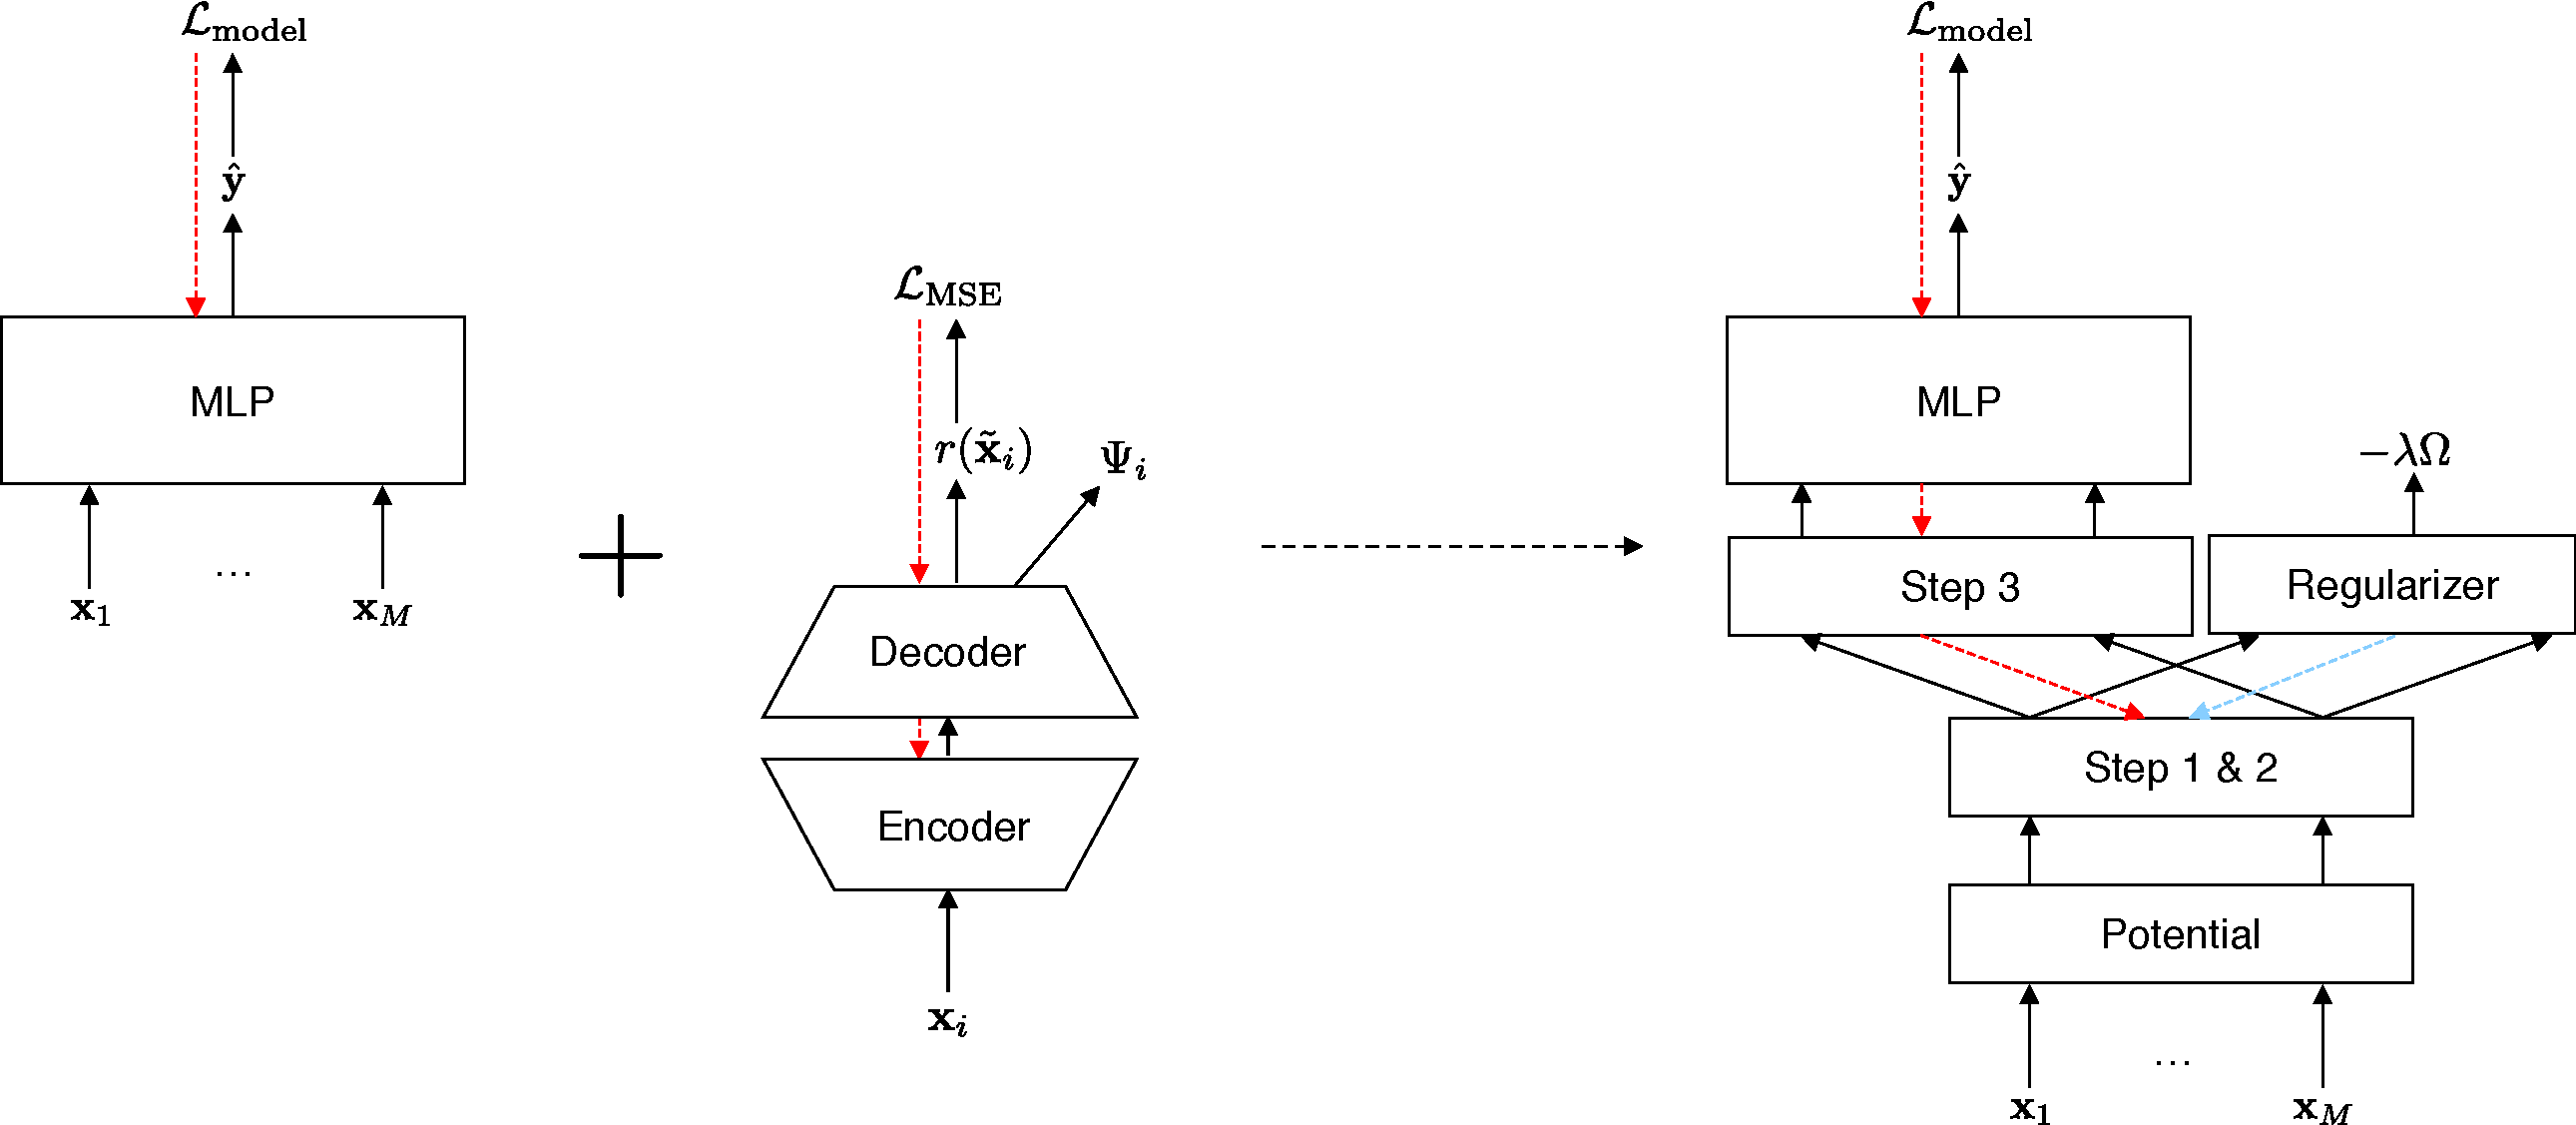
\includegraphics[scale=0.5]{figures/summary-training}
\caption{Summary of end-to-end training.}	
\label{fig:training}
\end{figure}
\end{center}
\vfill
\clearpage